
\documentclass{subfiles}

\begin{document}

\par FW LiDAR systems have been available for a number of years but there still very few users of FW LiDAR data. For example NERC-ARF has been acquiring FW LiDAR data since 2010 and despite that users show significant interest in acquiring those data, most research has focused on discrete LiDAR data. Some of the factors regarding this slow intakes are:

\begin{itemize}
	\item 
\end{itemize}

	\par {\color{red} *** the following paragraph is Dan and needs to be paraphrased}
Despite the availability of FW LiDAR systems for a number of years there are still very few users of FW data. For example, the Natural Environment Research Council Airborne Research Facility (NERC-ARF) has been acquiring FW data for the UK and overseas since 2010 and despite significant interest by users in having these data acquired, most research has focused on discrete data. The slow uptake of FW data is due to a number of factors: Existing workflows are only able to work with the discrete data since the increased amount of information recorded within the FW LiDAR makes handling the quantity of data very challenging. Typically FW datasets are 5 – 10 times larger than discrete data, with data sizes in the region of 50 – 250 GB for a single flight and up to 2TB for the entire area of interest.




	\par {\color{red} *** the following text has been taken from the IAA2 funding application}
	
\par To address the limitations of existing tools for working with FW data we developed the open source software DASOS ($\delta \alpha \sigma o \varsigma$=forest in Greek) and novel algorithms that allow users, without computer science expertise, to work with and visualise large volumes of FW LiDAR data. Our open source software DASOS aims to remove the barriers preventing the use of FW LiDAR. Its contributions, and those of the new representations of the FW LiDAR, are demonstrated in 
three applications:

\begin{itemize}
\item Firstly, foresters can exploit their domain expertise to derive a wealth of information by observing the FW LiDAR data. We therefore improve visualisations for deriving information directly from the data, thus reducing travelling time and the associated expenses of getting into the forests. This cost includes appropriate cars and sometimes helicopters depending on the accessibility of the forests. While previous work on FW LiDAR visualisation talks about point cloud visualisation (Isenburg, 2012) and transparent voxels (Persson et al, 2005), DASOS is able to reconstruct the surfaces from the scanned area in 3D. This research further optimisesvisualisations by using the new FW LiDAR representations to accelerate this process by up to****\% so far.

\item Secondly, a new and fast way of aligning the FW LiDAR with Remotely Sensed Images has been developed in DASOS. Subsequently, by generating tree coverage maps, it has been shown that the combination of these datasets confers better remote survey results (Miltiadou, 2015).

\item Finally, DASOS allow the generation of 3D signatures. An example usage of this information is characterising dead standing Eucalyptuses in Australia. Dead Eucalyptuses, from a biodiversity perceptive, are highly beneficial in native Australian forests since they are likely to be aged and have hollows. Many arboreal mammals and birds make use of these for shelters (Lindenmayer and Wood, 2010). Unfortunately, recent studies have shown that there is likely to be a shortage of hollows available for colonisation in the near future (Goldingay, 2009) (Gibbons and Lindenmayer, 2002). This is work in progress and a comparison between the discrete and FW LiDAR will be performed to demonstrate the increased survey accuracy obtained when the FW LiDAR is used.

\end{itemize}

\par There are currently over 100 users of new or archived NERC-ARF data, many of these have expressed an interest in working with FW LiDAR data.

\par In summary, FW LiDAR has great potential to improving automated surveying accuracy and consequently reduce the expensive fieldwork conducted in forestry. 

 and this research has already started to have an impact in the FW LiDAR community. DASOS is now used at Interpine Group Ltd, a world leading Forestry Company in New Zealand, and a PhD student at Bournemouth University is evaluating it for use in the estimation of bird distributions in the New Forest in the UK.

	
	\par {\color{red} *** end of copied text}
	




\begin{figure}
	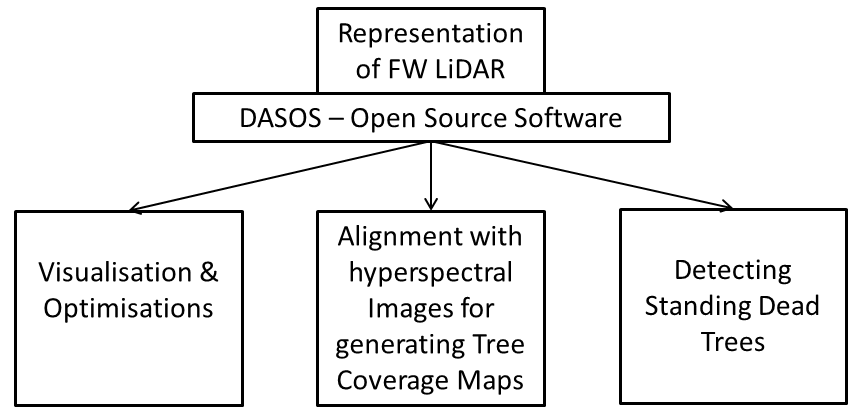
\includegraphics[width=\textwidth]{tex/Pipeline/Pipeline.png}
	\caption{The pipeline of the thesis}
\end{figure}


\section {Aims and Objectives}

The overarching aim of future work is to improve and optimise visualisations of full-waveform LiDAR data and hyperspectral images for remote forest surveying.

Objectives:\newline
1.	Enable browsing of very large scale datasets with many points and spectral bands in an efficient manner
2.	Estimate tree coverage and investigate the potential of integrating multiple remote sensing datasets in forestry
3.	Tree crown detection and height estimations in comparison to human detection, which will benefits wood trade and forest management
4.	Enable experts to establish wood coverage 
5.	Enable understanding of forestry concepts through 3D visualisations
6.	Investigate data structures that will be better for volumetric rendering and efficient management of large point clouds

This project explores visualisation and data-understanding for full waveform LIDAR systems. 

- How can large full waveform datasets be effectively and efficiently visualised? (especially in combination with other forms of data, such as hyperspectral images).
- How can terrain classification systems can be modified to effectively make use of full-waveform data? (for example, detection of dead trees for protecting animals living inside dead trees in Australia).  
- Can visualisation and classification be improved by inference of high quality 3D information, for example, using priors over the space of 3D elements and compatibility between multiple observations?
The project will also encompass other facets of large volume environmental dataset visualisation and understanding as appropriate.



\end{document}


